% \documentclass[professionalFonts,aspectratio=169]{beamer}
\documentclass[professionalFonts]{beamer}

\usepackage{beamerthemesplit}
\setbeamersize{text margin left=0.1em}  % <- like this
\setbeamersize{text margin right=0.1em} % <- like this


\usepackage[latin1]{inputenc}
\usetheme{Madrid}
\usecolortheme{rose}
% \usepackage{listings}
% \usepackage{fourier}
% \usepackage[scaled=0.8]{luximono}
\usepackage{helvet}
\usepackage{ulem}

\title[Writing a Mini-Lisp Compiler]{%
  Writing a Mini-Lisp Compiler
}
\author{Carlo Hamalainen}
\institute{carlo-hamalainen.net}
\date{28 May 2013}



\newenvironment{changemargin}[2]{% 
  \begin{list}{}{% 
    \setlength{\topsep}{0pt}% 
    \setlength{\leftmargin}{#1}% 
    \setlength{\rightmargin}{#2}% 
    \setlength{\listparindent}{\parindent}% 
    \setlength{\itemindent}{\parindent}% 
    \setlength{\parsep}{\parskip}% 
  }% 
  \item[]}{\end{list}} 

% Taken from http://widerin.org/blog/syntax-highlighting-for-python-scripts-in-latex-documents
\usepackage{color}
\usepackage{listings}
\usepackage{setspace}
\usepackage{fancyvrb}

\definecolor{Code}{rgb}{0,0,0}
\definecolor{Decorators}{rgb}{0.5,0.5,0.5}
\definecolor{Numbers}{rgb}{0.5,0,0}
\definecolor{MatchingBrackets}{rgb}{0.25,0.5,0.5}
\definecolor{Keywords}{rgb}{0,0,1}
\definecolor{self}{rgb}{0,0,0}
\definecolor{Strings}{rgb}{0,0.63,0}
\definecolor{Comments}{rgb}{0,0.63,1}
\definecolor{Backquotes}{rgb}{0,0,0}
\definecolor{Classname}{rgb}{0,0,0}
\definecolor{FunctionName}{rgb}{0,0,0}
\definecolor{Operators}{rgb}{0,0,0}
\definecolor{Background}{rgb}{0.98,0.98,0.98}

\definecolor{lightblue}{rgb}{0.68, 0.85, 0.9}
\definecolor{lightgray}{rgb}{0.83, 0.83, 0.83}
\definecolor{lemon}{rgb}{1.0, 0.97, 0.0}
\definecolor{mintgreen}{rgb}{0.6, 1.0, 0.6}

\definecolor{red}{rgb}{1, 0.0, 0.0}
\definecolor{blue}{rgb}{0.0, 0.0, 1.0}

% Python style for highlighting
\newcommand\pythonstyle{\lstset{
%numbers=left,
%numberstyle=\footnotesize,
%numbersep=1em,
xleftmargin=1em,
framextopmargin=2em,
framexbottommargin=2em,
showspaces=false,
showtabs=false,
showstringspaces=false,
%frame=l,
tabsize=4,
% Basic
basicstyle=\ttfamily\small\setstretch{1},
backgroundcolor=\color{Background},
language=python,
% Comments
commentstyle=\color{Comments}\slshape,
% Strings
stringstyle=\color{Strings},
morecomment=[s][\color{Strings}]{"""}{"""},
morecomment=[s][\color{Strings}]{'''}{'''},
% keywords
morekeywords={import,from,class,def,for,while,if,is,in,elif,else,not,and,or,print,break,continue,return,True,False,None,access,as,,del,except,exec,finally,global,import,lambda,pass,print,raise,try,assert},
keywordstyle={\color{Keywords}\bfseries},
% additional keywords
morekeywords={[2]@invariant},
keywordstyle={[2]\color{Decorators}\slshape},
emph={self},
emphstyle={\color{self}\slshape},
%
}}


% Python environment
\lstnewenvironment{python}[1][]
{
\pythonstyle
\lstset{#1}
}
{}

% Python for external files
\newcommand\pythonexternal[1]{{
\pythonstyle
\lstinputlisting{#1}}}

% Python for inline
\newcommand\pythoninline[1]{{\pythonstyle\lstinline!#1!}}

\begin{document}

\begin{frame}
\titlepage
\end{frame}

\section{Introduction}

\begin{frame}

About 13 years ago I did an BSc/BInfTech combined degree.
\vspace{\baselineskip}

A few of the IT subjects were fun:
\vspace{\baselineskip}

\begin{itemize}

\item Computational complexity. NP-complete, etc.

\item Operating systems. We wrote our own memory pager in C.

\item Functional programming. Gofer on MS-DOS.

\item Compilers. We wrote a compiler for a mini-Java language, in C. 

\end{itemize}



\end{frame}

\begin{frame}

\begin{center}
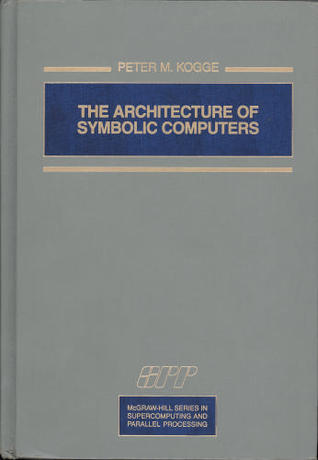
\includegraphics[width=4cm]{kogge.jpg}
\end{center}

The Architecture of Symbolic Computers (Peter M. Kogge, 1991)

\end{frame}

\begin{frame}

The Architecture of Symbolic Computers (Peter M. Kogge, 1991)
\vspace{\baselineskip}

{\small \url{http://blog.fogus.me/2012/07/25/some-lisp-books-and-then-some/}}
\vspace{\baselineskip}

``The best Lisp book I've ever read and could ever possibly read.''
\vspace{\baselineskip}

\url{http://www.loper-os.org/?p=13}
\vspace{\baselineskip}

``The Architecture of Symbolic Computers (Peter M. Kogge) is quite
possibly the most useful resource I have come across in my quest thus
far. If you are interested in Lisp Machine revival, non-von Neumann
computation, or the dark arts of the low-level implementation of
functional programming systems, you will not be disappointed.''


\end{frame}




\begin{frame}

Here's the plan:

\begin{enumerate}

\item Define a virtual machine: memory, registers, opcodes.
\item Write an emulator.
\item Define a mini-Lisp language (let, lambdas, etc).
\item Write a compiler for mini-Lisp to the virtual machine.
% \item Think about how to do IO.
\end{enumerate}

\end{frame}


\begin{frame}{IBM 704/709 - circa 1950}

16K per box!

\begin{center}
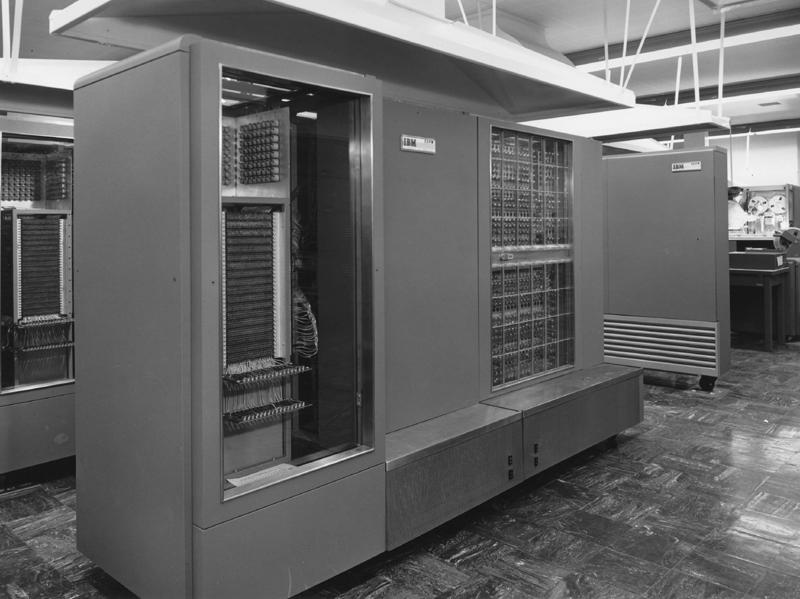
\includegraphics[width=7cm]{IBM704a.jpg}
\end{center}

{\small \url{http://www.computer-history.info/Page4.dir/pages/IBM.704.dir/}}

\end{frame}

\begin{frame}{IBM 704/709 - circa 1950}

Operator console.

\begin{center}
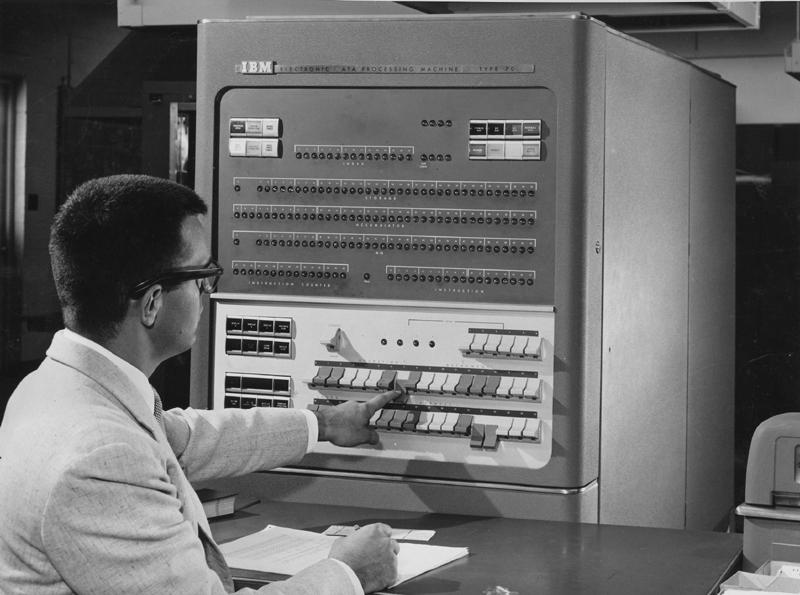
\includegraphics[width=7cm]{IBM704b.jpg}
\end{center}


{\small \url{http://www.computer-history.info/Page4.dir/pages/IBM.704.dir/}}

\end{frame}

% \begin{frame}{IBM 704/709 - circa 1950}
% 
% IBM 709 console:
% 
% \begin{center}
% 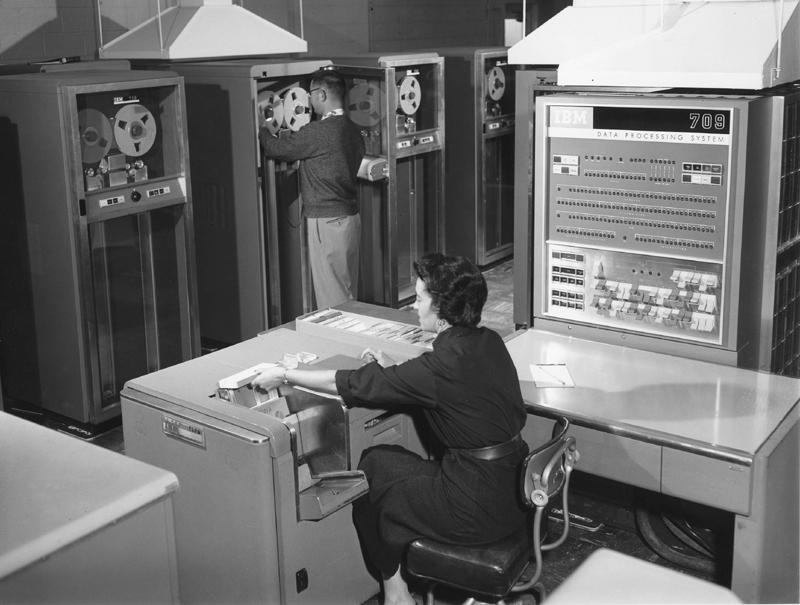
\includegraphics[width=7cm]{IBM709.jpg}
% \end{center}
% 
% 
% {\small \url{http://www.computer-history.info/Page4.dir/pages/IBM.704.dir/}}
% 
% \end{frame}


\begin{frame}{IBM 701 console}

\begin{center}
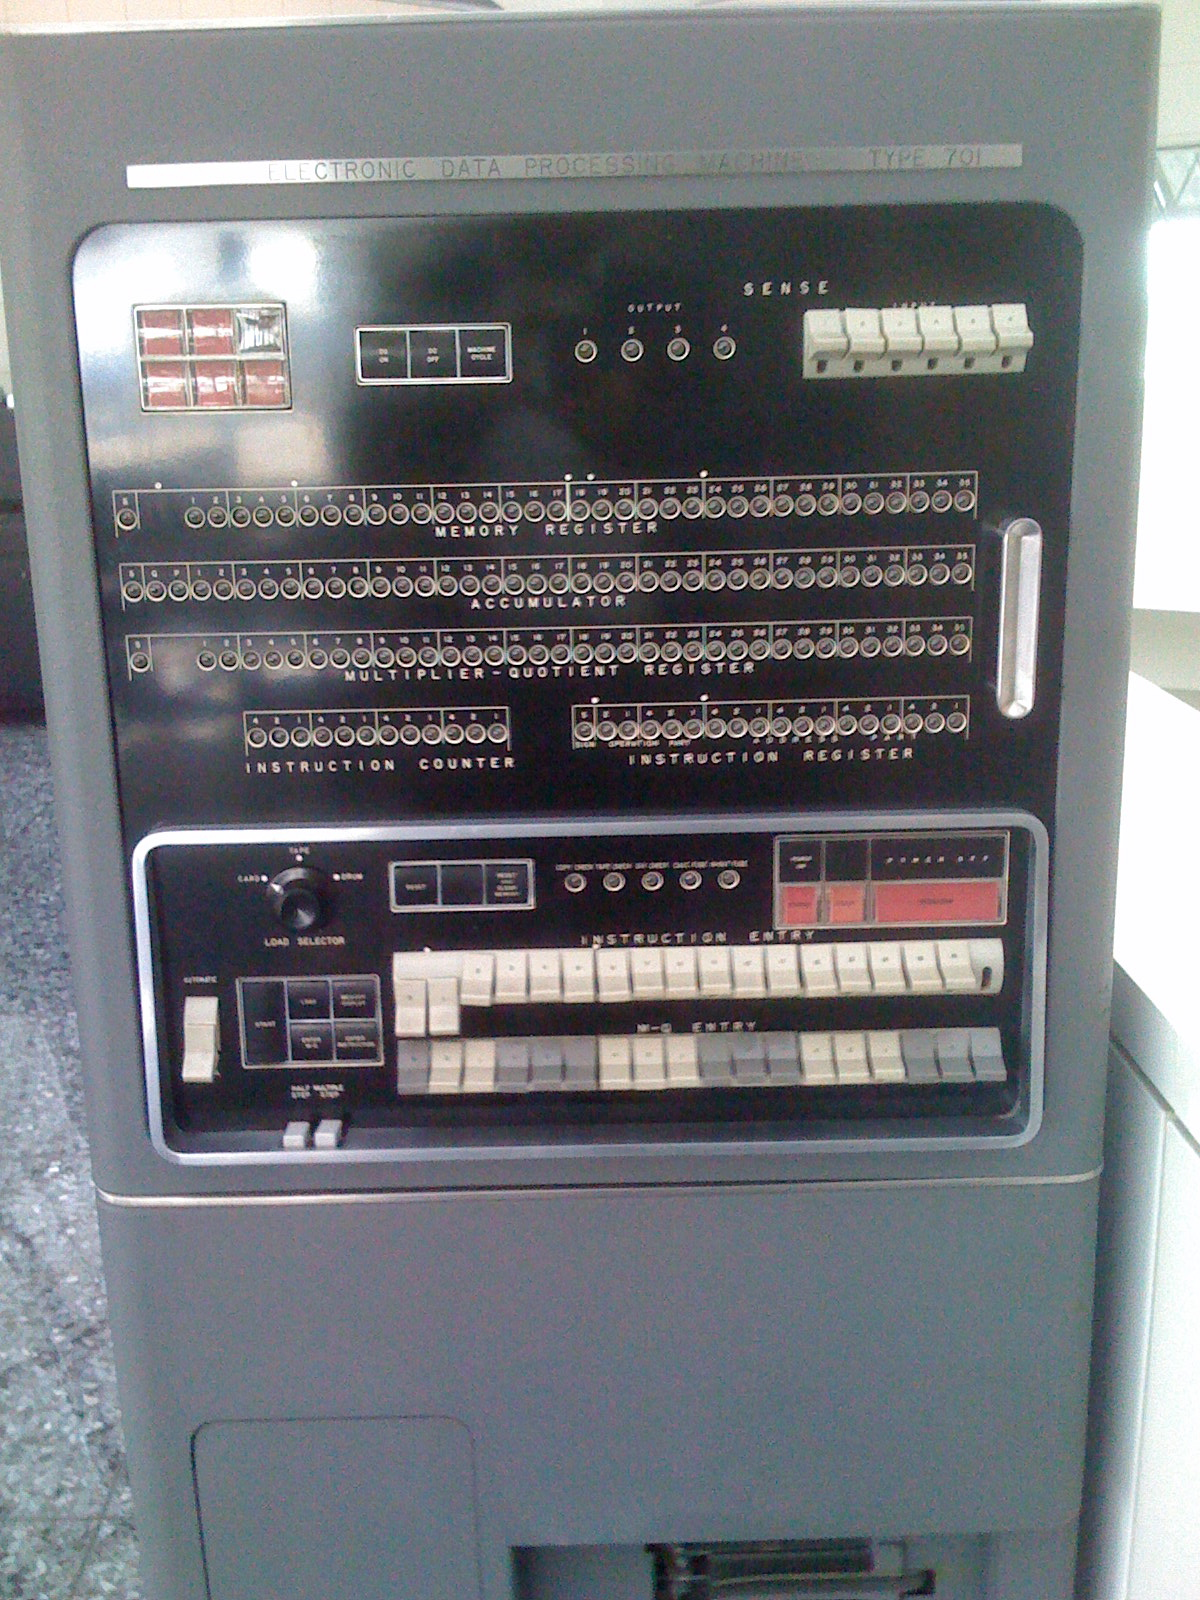
\includegraphics[width=8cm]{IBM_701console.jpg}
\end{center}


{\small \url{http://www.computer-history.info/Page4.dir/pages/IBM.704.dir/}}

\end{frame}


\begin{frame}

The IBM 704 had 36-bit machine words:

\begin{itemize}
\item address part: 15 bits
\item decrement part: 15 bits
\item prefix part: 3 bits
\item tag part: 3 bits
\end{itemize}

Corresponding instructions:

\begin{itemize}
\item CAR: Contents of Address part of Register
\item CDR: Contents of Decrement part of Register
\end{itemize}

Think of CAR as head and CDR as tail. Store linked lists with ease.

\end{frame}

\begin{frame}[fragile]

% \begin{python}[escapechar=!]
% [!\colorbox{mintgreen}{1}!, !\colorbox{mintgreen}{2}!, !\colorbox{mintgreen}{3}!]
% \end{python}

Store this list: 
\begin{python}[escapechar=!]
[!\color{blue}{1}!, !\color{blue}{2}!, !\color{blue}{3}!]
\end{python}

\begin{python}[escapechar=!]
address | value
---------------------
!\color{red}{5}!       | (6, 7)
!\color{red}{6}!       | !\color{blue}{1}!
!\color{red}{7}!       | (8, 9)
!\color{red}{8}!       | !\color{blue}{2}!
!\color{red}{9}!       | (10, 11)
!\color{red}{10}!      | !\color{blue}{3}!
!\color{red}{11}!      | (nil, nil)
\end{python}


\vspace{-3cm}
\begin{center}
\hspace{3cm}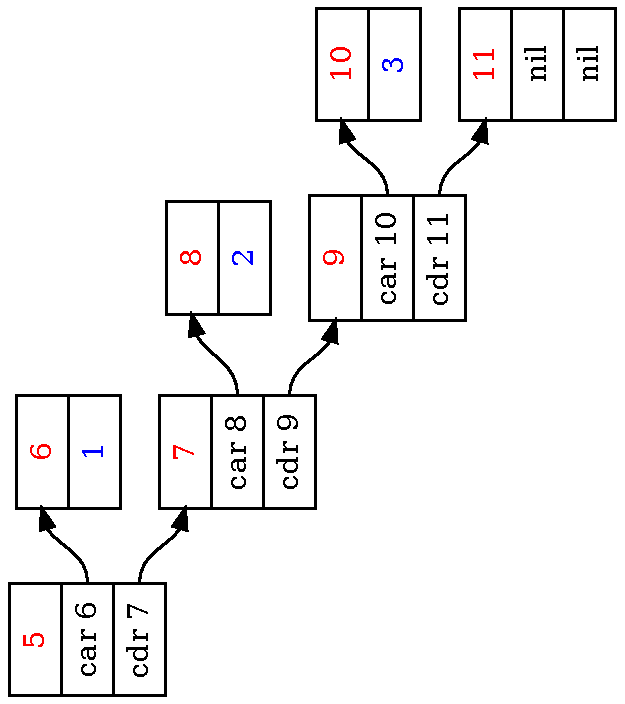
\includegraphics[angle=-90,origin=c,width=5cm]{list123.pdf}
\end{center}

% \vspace{-2cm}
% \pythoninline{car = head}\\
% \pythoninline{cdr = tail}\\
% \pythoninline{head . tail = car . cdr = cadr}\\
% \pythoninline{head . tail . tail = car . cdr . cdr = caddr}\\

\end{frame}

\begin{frame}[fragile]

\begin{python}
[LDC, [3, 4], LDF, [LD, [1, 2], LD, [1, 1], ADD, RTN],
              AP, WRITEI, STOP,]
\end{python}

\begin{center}
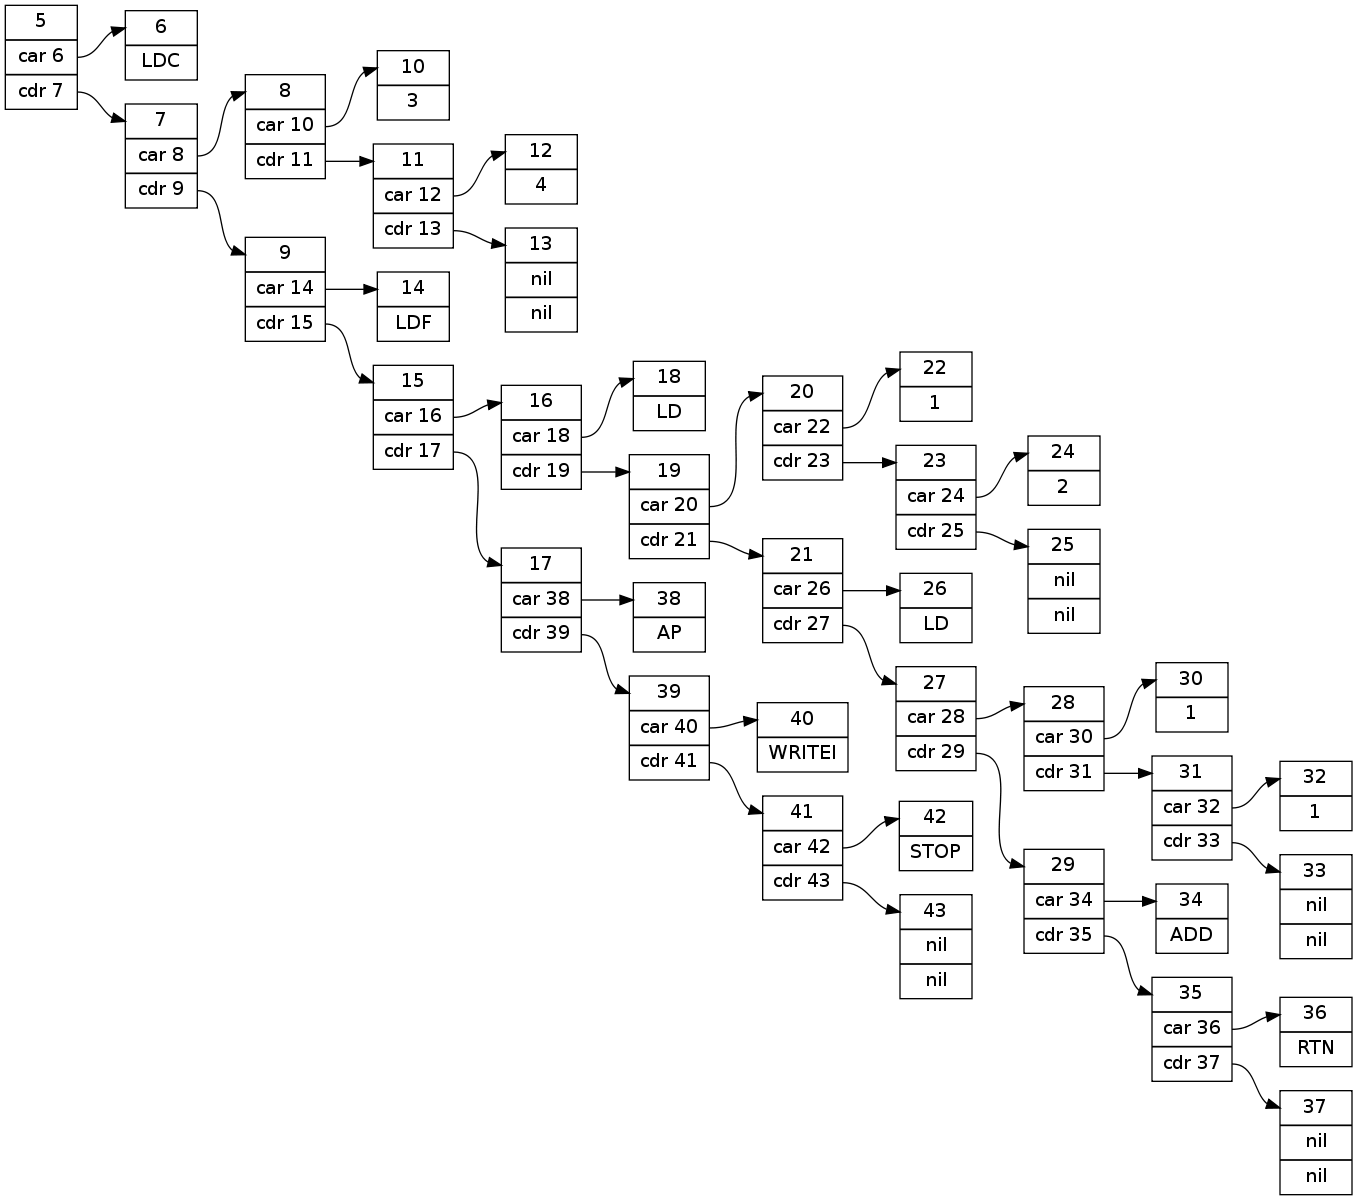
\includegraphics[width=8cm]{program_in_memory.png}
\end{center}

\end{frame}

\begin{frame}

A linked list can represent a stack:

\begin{itemize}

\item push: insert at front, return new head.
\item pop: remove from front, return cdr (tail) of original head.

\end{itemize}

% We can model computation with a stack:
% 
% \begin{itemize}
% \item Stack: \pythoninline{[]}
% 
% \item Push 3.  Stack: \pythoninline{[3]}
% 
% \item Push 4.  Stack: \pythoninline{[4, 3]}
% 
% \item Push ADD.  Stack: \pythoninline{[ADD, 4, 3]}
% 
% \item Execute ADD.  Stack: \pythoninline{[7]}
% 
% 
% \end{itemize}

We can run simple computations if we have two things:

\begin{itemize}

\item A stack for temporary results (like an accumulator register); and
\item a pointer to the next instruction to execute.
\end{itemize}


\end{frame}

\begin{frame}[fragile]

\begin{itemize}

\item S: temporary results stack.

\item C: program counter for currently executing code.

\item \pythoninline{LDC}: LoaD Constant
\item \pythoninline{ADD}: integer ADDition
\item \pythoninline{STOP}: STOP the machine
\end{itemize}

Add 3 and 4:

\begin{python}
1. S: []       C: [LDC, 3, LDC, 4, ADD, STOP]

2. S: [3]      C: [LDC, 4, ADD, STOP]

3. S: [4, 3]   C: [ADD, STOP]

4. S: [7]      C: [STOP]
\end{python}

\end{frame}

\begin{frame}[fragile]

\begin{python}
LDC  = 100
ADD  = 101
STOP = 102

S = []
C = [LDC, 3, LDC, 4, ADD, STOP]

def opcode_LDC(S, C):
    assert C[0] == LDC
    C.pop(0)              # pop LDC
    S.insert(0, C.pop(0)) # push value onto S

def opcode_ADD(S, C):
    assert C[0] == ADD
    C.pop(0)                 # pop ADD
    val1 = S.pop(0)          # first value
    val2 = S.pop(0)          # second value
    S.insert(0, val1 + val2) # push result
\end{python}

\end{frame}

\begin{frame}[fragile]
Here's the machine emulator:

\begin{python}
S = []
C = [LDC, 3, LDC, 4, ADD, STOP]

while True:
    if   C[0] == STOP: break
    elif C[0] == LDC:
        opcode_LCD(S, C)
    elif C[0] == ADD:
        opcode_ADD(S, C)
    else:
        assert False
\end{python}

\end{frame}

\begin{frame}[fragile]
Summary of the machine so far:

\begin{itemize}

\item Memory: a cell contains an integer or (car, cdr) tuple.

\item Registers: S (stack), C (code).

\item Opcodes: \pythoninline{ADD}, \pythoninline{LDC}, \pythoninline{STOP}.

\end{itemize}

This doesn't do much --- we need functions of some sort.

\end{frame}

\begin{frame}[fragile]

Lambda expressions:

\begin{itemize}

\item Python: \pythoninline{(lambda x, y: x + y)(3, 4)}

\item Haskell: \pythoninline{(\\x y -> x + y) 3 4}

\item Haskell': \pythoninline{(\\x y -> (+) x y) 3 4}

\item Lisp: \pythoninline{((LAMBDA (x y) (+ x y)) (3 4))}
\end{itemize}

Problems:

\begin{itemize}

\item Can't store ``x'', so remember \pythoninline{x = } first parameter, etc.

\item Save environment before call: new register D (dump).

\item Store arguments: new register E (environment).

\item New opcodes:

    \begin{itemize}
    \item LD: LoaD identifier. e.g. \pythoninline{[LD, 1] = } load value of \pythoninline{x}.
    \item LDF: LoaD Function. Push a closure onto S.
    \item AP: APply function. Evaluate a closure.
    \item RTN: ReTurN from function. Restore state.
    \end{itemize}

\end{itemize}


\end{frame}

%\begin{frame}[fragile]
%
%\begin{itemize}
%
%\item LD: LoaD identifier. e.g. \pythoninline{[LD, 1] = } load value of \pythoninline{x}.
%\item LDF: LoaD Function. Push a closure onto S.
%\item AP: APply function. Evaluate a closure.
%\item RTN: ReTurN from function. Restore state.
%\end{itemize}
%
%\pythoninline{(lambda x, y: x + y)(3, 4)}
%
%
%
%\begin{python}[escapechar=!]
%S: []
%C: [!\colorbox{lightgray}{LDC, [3, 4]}!, !\colorbox{mintgreen}{LDF, [LD, 2, LD, 1, ADD, RTN]}!, !\colorbox{lemon}{AP}!, STOP]
%\end{python}
%
%\end{frame}

\begin{frame}[fragile]
\begin{python}[escapechar=!]
S: []
E: []
C: [!\colorbox{lightgray}{LDC, [3, 4]}!, !\colorbox{mintgreen}{LDF, [LD, 2, LD, 1, ADD, RTN]}!, !\colorbox{lemon}{AP}!, STOP]
D: []
\end{python}

\begin{python}[escapechar=!]
S: [!\colorbox{lightgray}{[3, 4]}!]
E: []
C: [!\colorbox{mintgreen}{LDF, [LD, 2, LD, 1, ADD, RTN]}!, !\colorbox{lemon}{AP}!, STOP]
D: []
\end{python}

\begin{python}[escapechar=!]
S: [!\colorbox{mintgreen}{[LD, 2, LD, 1, ADD, RTN]}!, !\colorbox{lightgray}{[3, 4]}!]  # a closure
E: []
C: [!\colorbox{lemon}{AP}!, STOP]
D: []
\end{python}
\end{frame}

\begin{frame}[fragile]

\begin{python}[escapechar=!]
S: [!\colorbox{mintgreen}{[LD, 2, LD, 1, ADD, RTN]}!, !\colorbox{lightgray}{[3, 4]}!]  # a closure
E: []
C: [!\colorbox{lemon}{AP}!, STOP]
D: []
\end{python}

\begin{python}[escapechar=!]
S: []
E: [!\colorbox{lightgray}{[3, 4]}!]
C: !\colorbox{mintgreen}{[LD, 2, LD, 1, ADD, RTN]}!
D: [[S=[], E=[], C=[STOP]]
\end{python}

\begin{python}[escapechar=!]
S: [4]
E: [!\colorbox{lightgray}{[3, 4]}!]
C: !\colorbox{mintgreen}{[LD, 1, ADD, RTN]}!
D: [[S=[], E=[], C=[STOP]]
\end{python}
\end{frame}

\begin{frame}[fragile]
\begin{python}[escapechar=!]
S: [3, 4]
E: [!\colorbox{lightgray}{[3, 4]}!]
C: !\colorbox{mintgreen}{[ADD, RTN]}!
D: [[S=[], E=[], C=[STOP]]
\end{python}

\begin{python}[escapechar=!]
S: [7]
E: [!\colorbox{lightgray}{[3, 4]}!]
C: !\colorbox{mintgreen}{[RTN]}!
D: [[S=[], E=[], C=[STOP]]
\end{python}

\begin{python}[escapechar=!]
S: [7]
E: []
C: [STOP]
D: []
\end{python}
\end{frame}

\begin{frame}[fragile]
%\frametitle{Phew!}
%
%\begin{itemize}
%
%\item IBM 704/709 memory architecture makes it easy to store lists, stacks.
%
%\item Compute with stacks: \pythoninline{[LDC, 3, LDC, 4, ADD]}
%
%\item Code as code:
%
%\begin{python}[escapechar=!]
%C: [!\colorbox{mintgreen}{LDF, [LD, 2, LD, 1, ADD, RTN]}!, !\colorbox{lemon}{AP}!, STOP]
%\end{python}
%
%\item Code as data:
%
%\begin{python}[escapechar=!]
%S: [!\colorbox{mintgreen}{[LD, 2, LD, 1, ADD, RTN]}!, !\colorbox{lightgray}{[3, 4]}!]  # a closure
%\end{python}
%
%\end{itemize}

SECD machine summary so far:

\begin{itemize}

\item Memory: a cell contains an integer or (car, cdr) tuple.

\item Registers: S (stack), E (environment), C (code), D (dump).

\item Opcodes: \pythoninline{ADD}, \pythoninline{LDC}, \pythoninline{STOP} \pythoninline{LD}, \pythoninline{LDF}, \pythoninline{RTN}, \pythoninline{AP}.

\item Can evaluate lambda expressions.
\end{itemize}


\end{frame}

\begin{frame}[fragile]
\frametitle{SECD opcodes}
\begin{python}
ADD    # integer addition
MUL    # integer multiplication
SUB    # integer subtraction
DIV    # integer division

NIL    # push nil pointer onto the stack
CONS   # cons the top of the stack onto the next list
LDC    # push a constant argument
LDF    # load function
AP     # function application
LD     # load a variable
CAR    # value of car cell
CDR    # value of cdr cell

DUM    # setup recursive closure list
RAP    # recursive apply
\end{python}
\end{frame}

\begin{frame}[fragile]
\frametitle{SECD opcodes contd.}
\begin{python}
JOIN   # C = pop dump
RTN    # return from function
SEL    # logical selection (if/then/else)
NULL   # test if list is empty

WRITEI # write an integer to the terminal
WRITEC # write a character to the terminal

READC  # read a single character from the terminal
READI  # read an integer from the terminal

ZEROP # test if top of stack = 0 [nonstandard opcode]
GT0P  # test if top of stack > 0 [nonstandard opcode]
LT0P  # test if top of stack < 0 [nonstandard opcode]

STOP   # halt the machine
\end{python}
\end{frame}

\begin{frame}[fragile]

\frametitle{Final steps...}

\begin{itemize}

\item Define a simple Lisp language.

\item Write a function \pythoninline{compile(x)} to translate Lisp forms
into SECD machine code.

\end{itemize}


\end{frame}

\begin{frame}[fragile]

\frametitle{Square-bracket Lisp}

\begin{python}
# 3 + 4
[ADD, 3, 4]

# lambda x, y: x + y
[LAMBDA, ['x', 'y'], [ADD, 'x', 'y']]

# (lambda x, y: x + y)(3, 4)
[[LAMBDA, ['x', 'y'], [ADD, 'x', 'y']], 3, 4]

# x = 5; y = 7; x - y
[LET, ['x', 'y'], [5, 7], [SUB, 'x', 'y']]

\end{python}


\end{frame}

\begin{frame}[fragile]

\frametitle{Square-bracket Lisp}

\begin{python}
[ADD, 3, 4]

>>> compile([ADD, 3, 4])
[LDC, 4, LDC, 3, ADD, STOP]

def compile(x):
    if x[0] == ADD:
        x.pop(0)
        arg1 = x.pop(0)
        arg2 = x.pop(0)
        return [LDC, compile(arg1), \
                LDC, compile(arg2),
                ADD] \
                + compile(x)
    elif ...
\end{python}

\end{frame}


\begin{frame}[fragile]

\frametitle{Square-bracket Lisp}

\begin{python}
# lambda x, y: x + y
[LAMBDA, ['x', 'y'], [ADD, 'x', 'y']]

>>> compile([LAMBDA, ['x', 'y'], [ADD, 'x', 'y']])
[LDF, [LD, [1, 2], LD, [1, 1], ADD, RTN]]
\end{python}

\end{frame}

\begin{frame}[fragile]

\frametitle{Square-bracket Lisp}

\begin{python}
# (lambda x, y: x + y)(3, 4)
[[LAMBDA, ['x', 'y'], [ADD, 'x', 'y']], 3, 4]

>>> c = [[LAMBDA, ['x', 'y'], [ADD, 'x', 'y']], 3, 4]
>>> compile(c)
[NIL, LDC, 4, CONS, LDC, 3, CONS,
 LDF, [LD, [1, 2], LD, [1, 1], ADD, RTN],
 AP,
 STOP]

\end{python}

\end{frame}

\begin{frame}[fragile]
\frametitle{Square-bracket Lisp}

\begin{python}
# x = 5; y = 7; x - y
[LET, ['x', 'y'], [5, 7], [SUB, 'x', 'y']]

>>> c = [LET, ['x', 'y'], [5, 7], [SUB, 'x', 'y']]
>>> compile(c)
[NIL, LDC, 7, CONS, LDC, 5, CONS,
 LDF, [LD, [1, 2], LD, [1, 1], SUB, RTN],
 AP,
 STOP]

\end{python}

\end{frame}

\begin{frame}[fragile]

Length of a list?

\begin{verbatim}
> let f x m = if null x
                then m
                else f (tail x) (m + 1)
> f [1, 2, 3] 0
3
\end{verbatim}

\begin{python}
[LETREC, ['f'], [[LAMBDA, ['x', 'm'],
    [IF, [NULL, 'x'],
         'm',
         ['f', [CDR, 'x'], [ADD, 'm', 1]]]]],
  ['f', [LIST, 1, 2, 3], 0]
\end{python}
\end{frame}



\begin{frame}

Square-bracket Lisp:

\begin{itemize}

\item Enough to write basic programs: \pythoninline{LET}, \pythoninline{LAMBDA}, \pythoninline{IF}.

\item Recursion using \pythoninline{LETREC}.

\item No destructive assignment: pure Lisp.

\item Closures can be evaluated in the future, always same value.

\item Code as data.

\item Lambda expressions $\leftrightarrow$ S-expressions.

\item Relies on machine to do garbage collection (say what?).

\end{itemize}

\end{frame}

\begin{frame}

The CURRY chip (Ramsdell, 1986)

\begin{itemize}
\item 0.4Mhz
\item CPU chip: about 9000 transistors, performed graph reduction (combinators S, K, I).
\item Memory chip: garbage collection.
\item Timing chip: overall timing and control console.
\end{itemize}

\begin{center}
\includegraphics[width=7cm]{curry_chip.png}
\end{center}

% TODO: Figure 11-31 on p. 332

\end{frame}

\begin{frame}

MultiLISP: parallel Lisp

\begin{itemize}

\item Pure lambda calculus $\Rightarrow$ opportunities for parallelism.

\item Concert machine at MIT: 24-way Motorola 68000-based shared-memory multiprocessor (early 80s?).

\item MultiLISP $\rightarrow$ SECD-like abstract machine called MCODE.

\item MCODE interpreter (3000 lines of C).

\item Unfortunately slow due to MCODE, but parallel benefits could be measured.

\item Used {\it futures} for evaluation; see also Swift: \url{http://www.ci.uchicago.edu/swift/main/}

\end{itemize}


\end{frame}

\begin{frame}

Symbolics Lisp Machine

\begin{center}
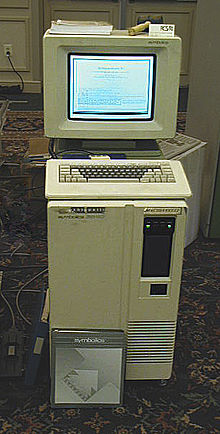
\includegraphics[width=4cm]{220px-Symbolics3640_Modified.JPG}
\end{center}

% TODO: detail from book

% Hardare garbage collection.

% Hardware type checking. % http://www.faqs.org/faqs/lisp-faq/part2/section-20.html

% quote from wikipedia on Symbolics: ``These machines had hardware
% support for various primitive Lisp operations (data type testing, CDR
% coding) and also hardware support for incremental garbage collection.''

\end{frame}

\begin{frame}

Symbolics Lisp Machine

\begin{itemize}

\item Instruction set: stack machine, similar to SECD.

\item Hardware support:

    \begin{itemize}
    \item virtual memory
    \item garbage collection
    \item data type testing
    \end{itemize}


\end{itemize}

\end{frame}

\begin{frame}

Symbolics Lisp Machine keyboard

\begin{center}
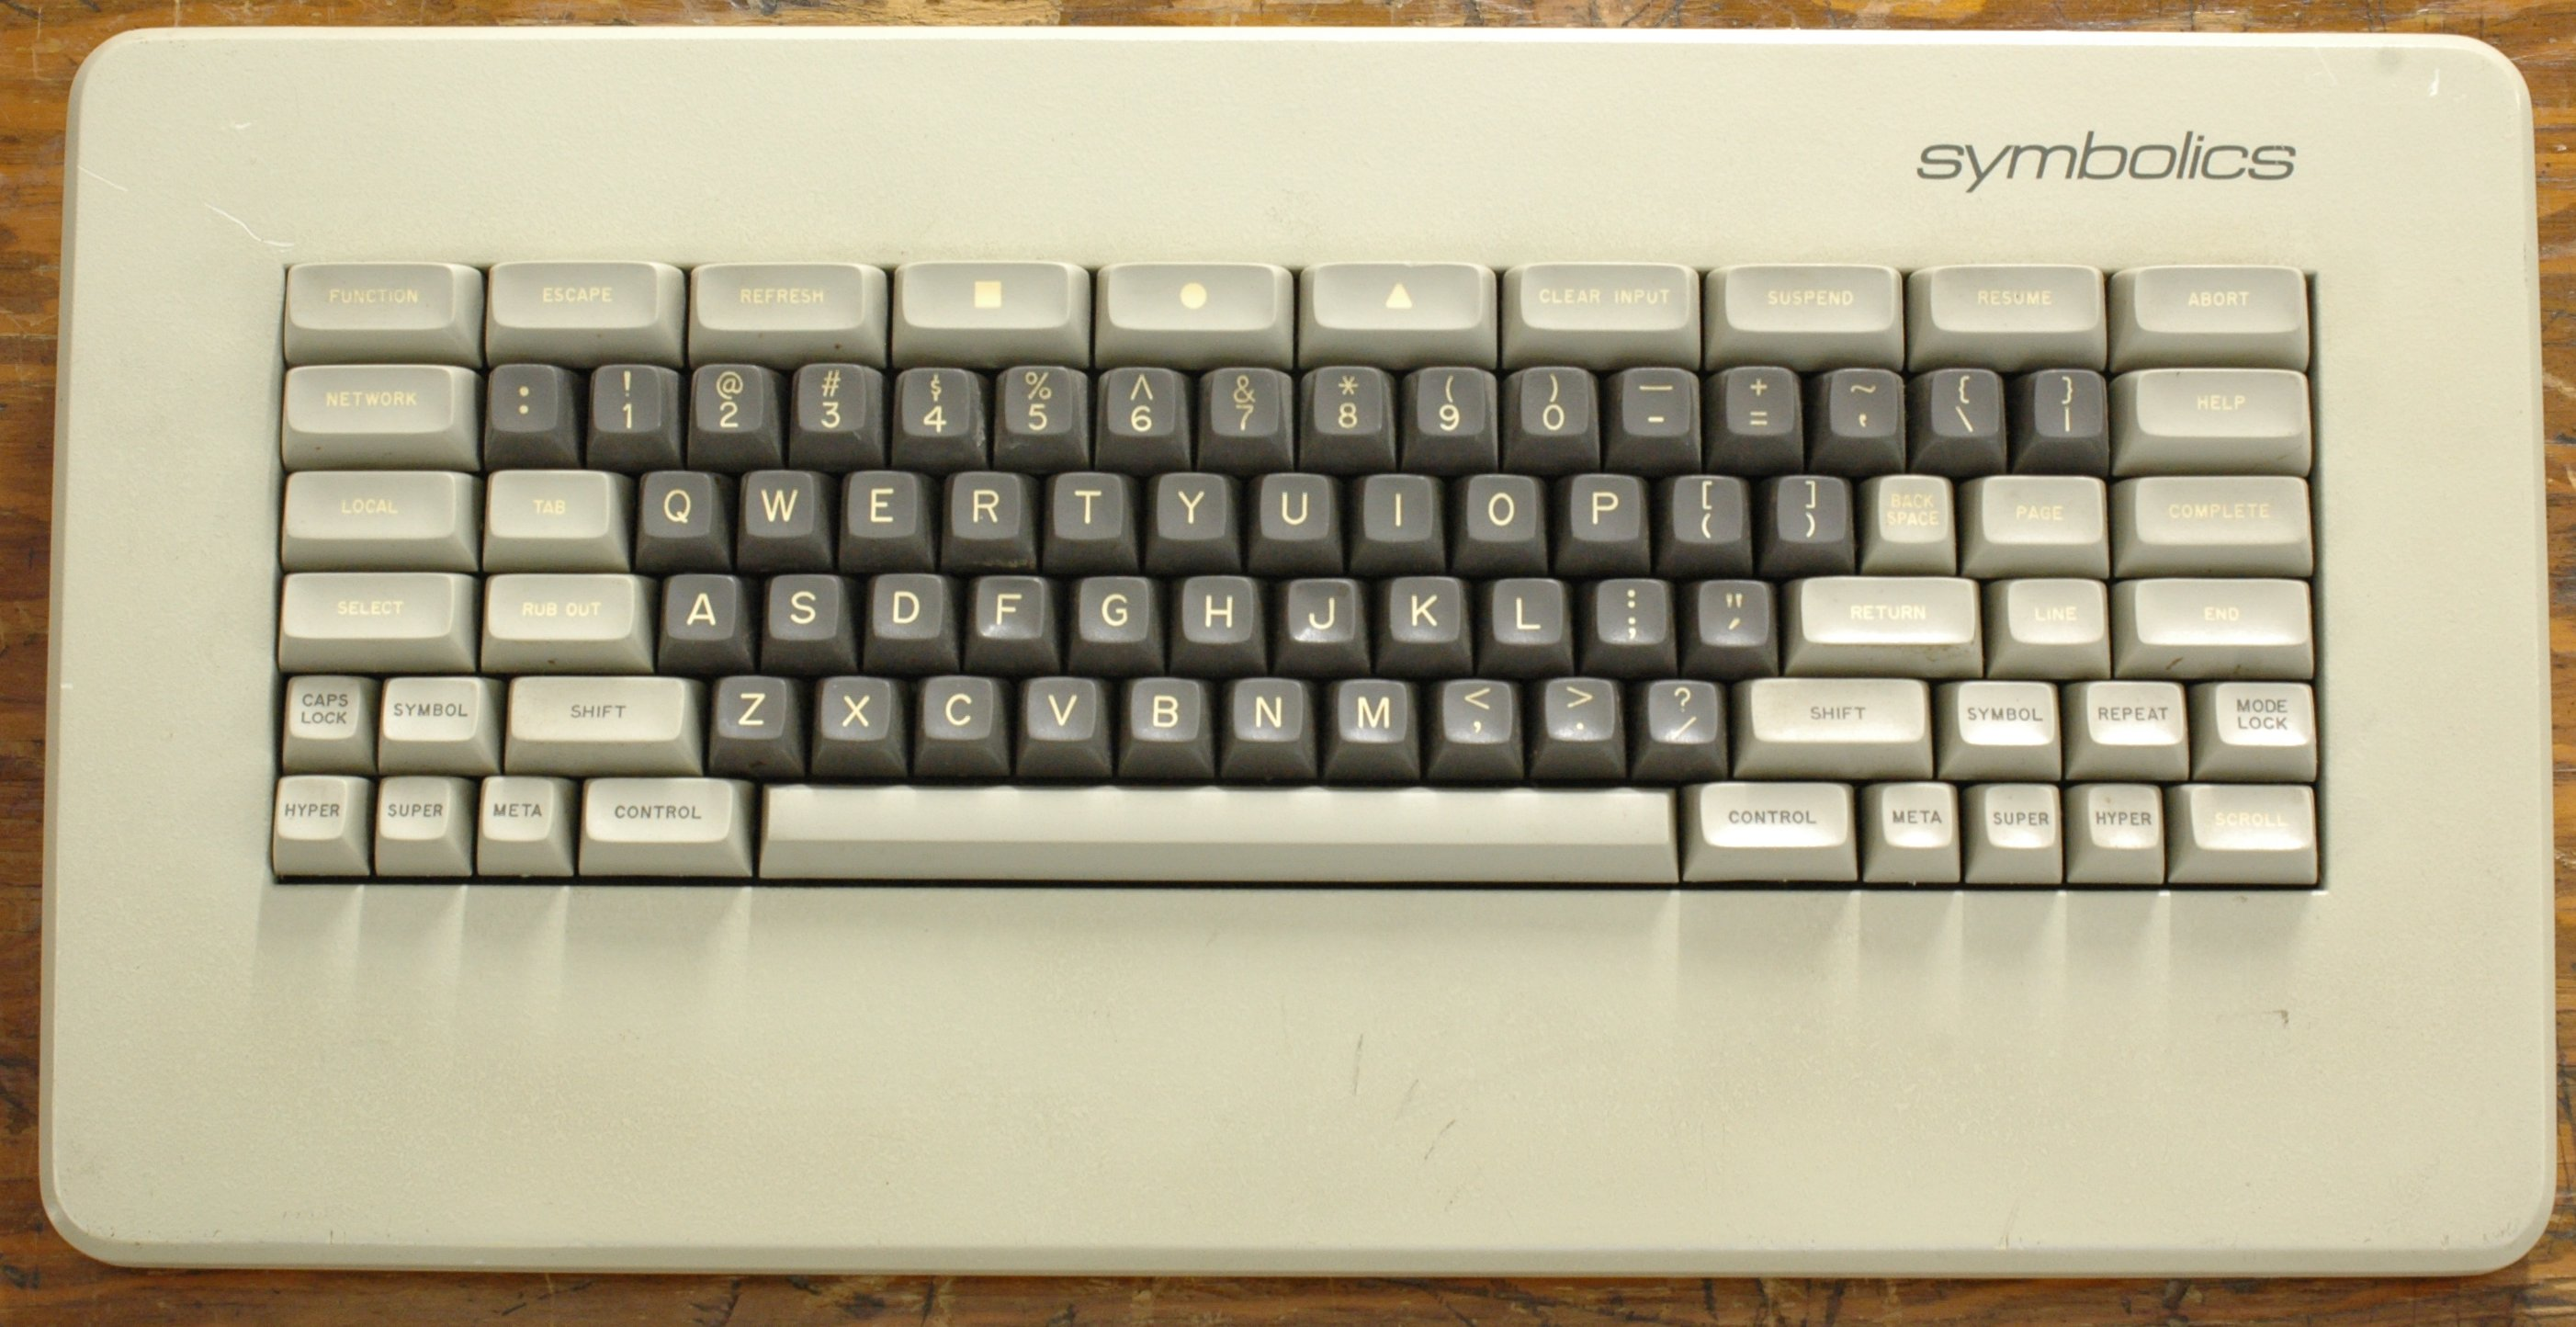
\includegraphics[width=12cm]{Symbolics-keyboard.jpg}
\end{center}

modifier keys: HYPER SUPER META CONTROL

\end{frame}

\begin{frame}[References]

My SECD emulator and mini-Lisp compiler: \url{https://github.com/carlohamalainen/pysecd}

\end{frame}

\end{document}

\begin{frame}[fragile]
\frametitle{Aside: a = 3; b = 4; a + b on Intel (FIXME: remove?)}
{\small
\begin{verbatim}
global _start
section .text
_start:
    ; a + b
    mov ebx, [a]    ; ebx = a
    add ebx, [b]    ; ebx += b
    ; exit; return value is ebx
    mov eax, 1
    int 80h

section .data
    a: db 0x3   ; a = 0x3
    b: db 0x4   ; b = 0x4

$ nasm -f elf64 -o add34.o add34.nasm && ld -o add34 add34.o
$ ./add34;  echo $?
7
\end{verbatim}
}
\end{frame}



\begin{frame}

Part II \\
\hspace*{12pt} Chapter 4 Lambda Calculus \\
\hspace*{12pt} Chapter 5 A Formal Basis for Abstract Programming \\
\hspace*{12pt} Chapter 6 Self-Interpretation \\
\hspace*{12pt} Chapter 7 The SECD Abstract Machine\\
\hspace*{12pt} Chapter 8 Memory Management for S-expressions \\
\hspace*{12pt} Chapter 9 Demand-Drive Evaluation \\
\hspace*{12pt} Chapter 10 LISP: Variations and Implementations\\
\hspace*{12pt} Chapter 11 Combinators and Graph Reduction\\
\hspace*{12pt} Chapter 12 Other Function-Based Computing Systems\\

\end{frame}


% TODO p. 119 Lambda expressions as s-expressions.


